\documentclass{article}%
\usepackage[T1]{fontenc}%
\usepackage[utf8]{inputenc}%
\usepackage{lmodern}%
\usepackage{textcomp}%
\usepackage{lastpage}%
\usepackage[head=40pt,margin=0.5in,bottom=0.6in]{geometry}%
\usepackage{graphicx}%
%
\title{\textbf{Incendio detuvo arranque de destiladora en Amuay}}%
\author{El Nacional}%
\date{07/03/2019}%
%
\begin{document}%
\normalsize%
\maketitle%
\textbf{URL: }%
http://www.el{-}nacional.com/noticias/petroleo/incendio{-}detuvo{-}arranque{-}destiladora{-}amuay\_273750\newline%
%
\textbf{Periodico: }%
EN, %
ID: %
273750, %
Seccion: %
Petróleo\newline%
%
\textbf{Palabras Claves: }%
NO\_TIENE\newline%
%
\textbf{Derecho: }%
2.1%
, Otros Derechos: %
\newline%
%
\textbf{\textit{La plamta no logró reanudar operaciones tras el incidente ocurrido el martes, lo que limita las labores de procesamiento de crudo}}%
\newline%
\newline%
%
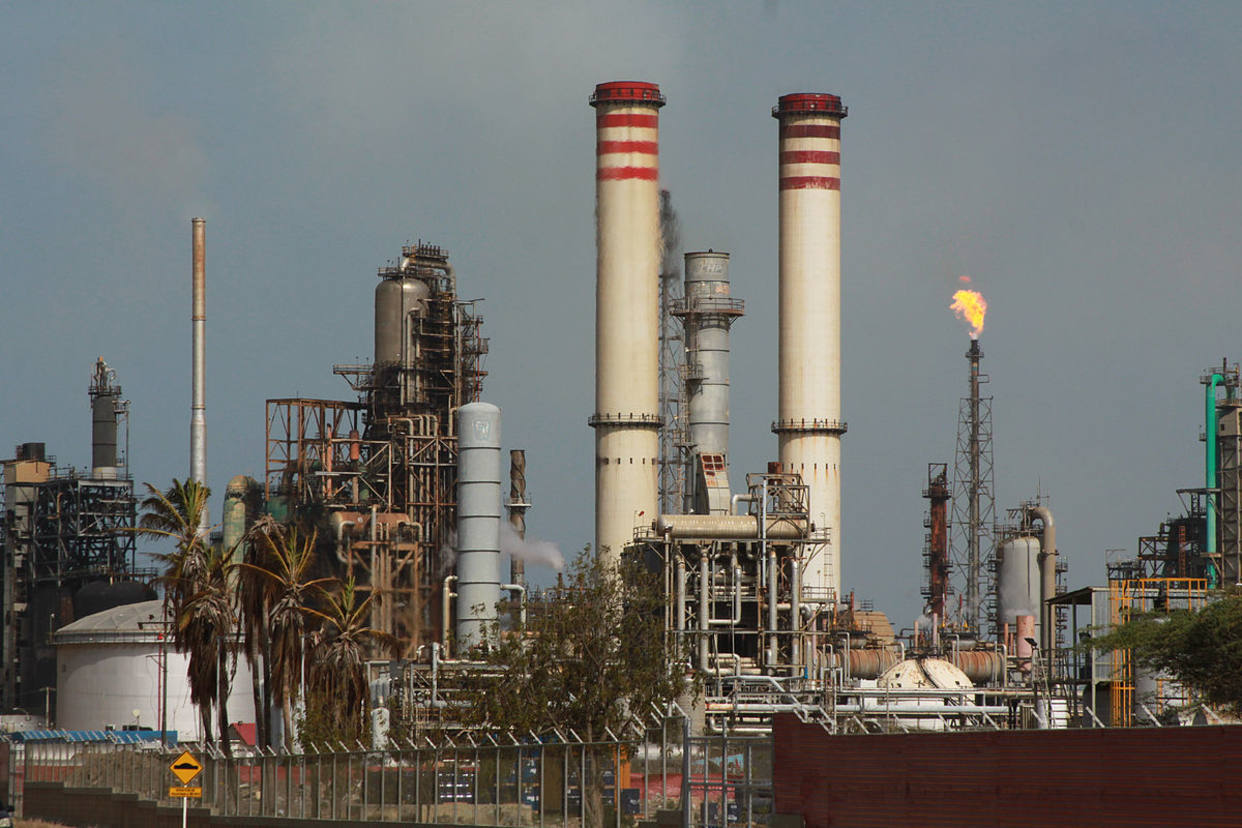
\includegraphics[width=300px]{EN_273750.jpg}%
\newline%
%
Un incendio detuvo esta semana el arranque de una unidad destiladora de la refinería de Azuay, la más importante de Venezuela, de acuerdo con lo declarado por un representante sindical y un trabajador del complejo.%
\newline%
%
La planta de destilación número 5 de la refinería, con capacidad para procesar 645.000 barriles por día (bpd) de petróleo, no logró reanudar operaciones tras el incidente ocurrido el martes, lo que limita las labores de procesamiento de crudo, apuntaron las fuentes.%
\newline%
%
La estatal Petróleos de Venezuela no respondió de inmediato una petición de comentario. Otras unidades de Amuay, como la planta de craqueo catalítico, se encontrarían también paralizadas.%
\newline%
%
“En medio de la desesperación por producir, querían arrancar esa planta y se produjo un incendio”, dijo el líder sindical Iván Freites.%
\newline%
%
Un trabajador del Complejo Refinador de Paraguaná, donde opera Amuay, confirmó el incidente en la planta destiladora “en pleno proceso de arranque, luego de estar detenida largo tiempo por una reparación”, según agregó a condición de preservar su anonimato.%
\newline%
%
El CRP, integrado por las refinerías de Amuay y Cardón, es uno de los mayores complejos del mundo, con capacidad para procesar hasta 955.000 bpd.%
\newline%
%
No obstante, según Freites, el circuito refinador operaba en mínimos esta semana, una vez que Amuay está produciendo unos 70.000 bpd y Cardón otros 40.000 bpd.%
\newline%
%
Con información de Reuter%
\newline%
%
\end{document}